% \documentclass{report}
% 
% \usepackage{fancyhdr}
\usepackage{fourier-orns}
\usepackage{hyperref}%% To refrence links / jumps
\usepackage{chngcntr} %% For some extra counters numberings
\usepackage[a4paper, right = 0.5in, left = 0.5in,top = 1in , bottom = 1in]{geometry}
\usepackage{etoolbox} %% Provides like a language for advanced customization
\usepackage{datetime} %% For dates of course
\usepackage{lastpage} %% provides pages numbers
\usepackage[sc]{titlesec} %% modify titles
\usepackage{enumerate}
\usepackage{cancel}
\usepackage{tikzsymbols}
\usepackage[dvipsnames]{xcolor}
\usepackage{import}
\usepackage{pdfpages} %% include other pdfs
\usepackage{transparent} %% Transparency
\usepackage{xcolor}  %% Colors
\usepackage[many]{tcolorbox}
\usepackage[framemethod=TikZ]{mdframed}
\usepackage{amsmath,amsfonts,amsthm,amssymb,mathtools}
\usepackage{tikz}
\usepackage{bookmark}
\usepackage{graphicx}
\usepackage{mathpazo}

\usepackage{fontawesome5}

\linespread{1.5}


\titleformat{\chapter}[display]   
{\fontfamily{ppl}\selectfont\huge\color{YellowOrange!80!orange}} % Font style and size 
{\raggedleft\color{purple}\fontsize{70}{0pt}\selectfont\thechapter}   
{-1.5cm}    			                          % Space between the chapter number and title
{
	\begin{tikzpicture}[overlay]
		\node[anchor = west,yshift = 0.2cm,xshift = -1cm] {\fontsize{90}{20} $\int_{}^{} $};
		\node[yshift = 4cm, xshift = 17cm]   {\includegraphics[width = 4cm]{preview0}};
	\end{tikzpicture}
\hspace{1cm}\Huge\raggedright\MakeUppercase}

\titleformat{\section}[block]
{
\fontfamily{ppl}\selectfont\huge\color{YellowOrange!80!orange}
}
{
\color{purple}\fontsize{20}{0pt}\selectfont\thesection 
}
{0cm}
{
	\begin{tikzpicture}[overlay]
		\node[anchor = west,yshift = 0.2cm,xshift = -0.4cm, circle = 1pt] {};
	\end{tikzpicture}
}

\titlespacing*{\section}{0pt}{0.7cm}{1.5cm}


\newcommand{\divider}
{
	\begin{center}
	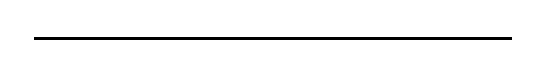
\begin{tikzpicture}
		\draw[thick, black] (0.25*\textwidth, 0) -- (0.75*\textwidth, 0);
		\node[rotate = 360 - 90, xshift = -0.6pt, yshift = 1pt] at (0.25*\textwidth,0){\decotwo};
		\node[rotate = 90, xshift = -0.6pt, yshift = 1pt] at (0.75*\textwidth,0){\decotwo};
	\end{tikzpicture}
	\end{center}
}

\pagestyle{fancy}

\newcommand{\lecday}[1][]
{
    \def\datee{#1}
    \fancyhead[L]{\datee}
}



\newcommand{\signature}
{
	\begin{tikzpicture}[remember picture,overlay]
		\node[fill = YellowOrange!20!white] at ([yshift = 1cm, xshift = -3cm]current page.south east) {\fontsize{10pt}{0pt}{\itshape Kara.$\mathcal{A}$}};
	\end{tikzpicture}
}

\AddToHook{shipout/background}{
  \begin{tikzpicture}[remember picture, overlay]
	  \node[] at ([yshift = 1.5cm,xshift = \textwidth /2 + 0.9cm]current page.south west) {\includegraphics[width = 0.5cm]{preview3}};
	  \node[] at ([yshift = 1.5cm,xshift = - \textwidth /2 - 0.9cm]current page.south east) {\includegraphics[width = 0.5cm]{preview4}};
  \end{tikzpicture}
}



\newtcolorbox[auto counter, number within = section]{remark}[1][]
{
       		title = Remark #1,
		enhanced,
		boxrule = 0pt,
		colback = white,
		breakable,
		arc = 4pt,
		colbacktitle = cyan,
		colback = cyan!5!white,
		segmentation style =
		{
			solid,cyan,thick,
		},
		attach boxed title to top left =
		{
			xshift = 0cm,
		},
		boxed title style =
		{
			boxrule = 0pt,
			sharp corners,
			drop fuzzy shadow = {cyan},
		},
		drop fuzzy shadow = {cyan!80!black},
}

\newtcolorbox[auto counter, number within = section]{theorem}[1][]
{                                      
		title = Theorem \thetcbcounter : #1,
		enhanced, 
		boxrule = 0pt,
		colback = white,
		breakable,
		arc = 4pt,
		colbacktitle = purple,
		colback = purple!5!white,
		segmentation style = 
		{
			solid, purple,thick,
		},
		attach boxed title to top left = 
		{
			xshift = 0cm, 
		},
		boxed title style = 
		{
			boxrule = 0pt,
			sharp corners,
			drop fuzzy shadow = {purple},
		},
		drop fuzzy shadow = {purple!80!black},
}

\newtcolorbox[auto counter, number within = section]{definition}[1][]
{                                      
		title = Definition \thetcbcounter : #1,
		enhanced, 
		boxrule = 0pt,
		colback = white,
		arc = 4pt,
		breakable,
		colbacktitle = YellowOrange!80!black,
		segmentation style = 
		{
			solid, YellowOrange,thick,
		},
		attach boxed title to top left = 
		{
			xshift = 0cm, 
		},
		colback = YellowOrange!5!white,
		boxed title style = 
		{
			boxrule = 0pt,
			sharp corners,
			drop fuzzy shadow = {YellowOrange!80!orange},
		},
		drop fuzzy shadow = {YellowOrange!80!black},
}

\newtcolorbox[auto counter, number within = section]{corollary}[1][]
{                                      
		title = corollary \thetcbcounter : #1,
		enhanced, 
		boxrule = 0pt,
		colback = white,
		arc = 4pt,
		breakable,
		colbacktitle = YellowOrange!80!black,
		segmentation style = 
		{
			solid, YellowOrange,thick,
		},
		attach boxed title to top left = 
		{
			xshift = 0cm, 
		},
		colback = YellowOrange!5!white,
		boxed title style = 
		{
			boxrule = 0pt,
			sharp corners,
			drop fuzzy shadow = {YellowOrange!80!orange},
		},
		drop fuzzy shadow = {YellowOrange!80!black},
}


\newtcolorbox{example}[1][]
{                                      
		title = Example,
		enhanced, 
		boxrule = 0pt,
		colback = white,
		arc = 4pt,
		segmentation style = 
		{
			solid, SpringGreen,thick,
		},
		breakable,
		colback = SpringGreen!5!white,
		colbacktitle = SpringGreen!80!black,
		attach boxed title to top left = 
		{
			xshift = 0cm, 
		},
		boxed title style = 
		{
			boxrule = 0pt,
			sharp corners,
			drop fuzzy shadow = {SpringGreen!80!orange},
		},
		drop fuzzy shadow = {SpringGreen!80!black},
}


\newcommand{\integral}[4]{\int\limits_{#1}^{#2} #4 d#3}
\newcommand{\limit}[3]{\lim\limits_{#1 \rightarrow #2} #3}
\newcommand{\strone}[2]{\left[ \begin{gathered}#1\\ #2\end{gathered} \right] }
\newcommand{\strtwo}[2]{\left\{ \begin{gathered}#1\\ #2\end{gathered} \right\} }
\newcommand{\strthree}[2]{\left\lfloor \begin{gathered}#1\\ #2\end{gathered} \right\rfloor }


\newcommand{\startbf}[1]{\text{\bfseries{#1}}}
\newcommand{\sett}[1]{\left\{ #1 \right\}}
\newcommand{\thesis}[1]{\left( #1 \right)}
\newcommand{\brkt}[1]{\left[ #1 \right]}
\newcommand{\floor}[1]{\left\lfloor #1 \right\rfloor}


\DeclareMathOperator{\img}{im} % Image
\DeclareMathOperator{\Img}{Im} % Image
\DeclareMathOperator{\coker}{coker} % Cokernel
\DeclareMathOperator{\Coker}{Coker} % Cokernel
\DeclareMathOperator{\Ker}{Ker} % Kernel
\DeclareMathOperator{\rank}{rank}
\DeclareMathOperator{\Spec}{Spec} % spectrum
\DeclareMathOperator{\Tr}{Tr} % trace
\DeclareMathOperator{\pr}{pr} % projection
\DeclareMathOperator{\ext}{ext} % extension
\DeclareMathOperator{\pred}{pred} % predecessor
\DeclareMathOperator{\dom}{dom} % domain
\DeclareMathOperator{\ran}{ran} % range
\DeclareMathOperator{\Hom}{Hom} % homomorphism
\DeclareMathOperator{\Mor}{Mor} % morphisms
\DeclareMathOperator{\End}{End} % endomorphism


\newcommand{\lm}{\ensuremath{\lambda}}
\newcommand{\eps}{\ensuremath{\epsilon}}
\newcommand{\veps}{\ensuremath{\varepsilon}}
\newcommand{\al}{\ensuremath{\alpha}}
\newcommand{\bb}{\ensuremath{\beta}}
\newcommand{\cc}{\ensuremath{\gamma}}
\newcommand{\dd}{\ensuremath{\delta}}
\newcommand{\DD}{\ensuremath{\Delta}}
\newcommand{\ff}{\ensuremath{\phi}}
\newcommand{\FF}{\ensuremath{\varphi}}

\newcommand{\RR}{\mathbb{R}}
\newcommand{\RO}{\mathcal{R}}
\newcommand{\EE}{\mathbb{E}}
\newcommand{\CC}{\mathbb{C}}
\newcommand{\RW}{\mathbb{R}^2}
\newcommand{\RT}{\mathbb{R}^3}
\newcommand{\RN}{\mathbb{R}^n}
\newcommand{\DS}{\mathcal{D}}

\newcommand{\KK}{\mathbb{K}}
\newcommand{\KW}{\mathbb{K}^2}
\newcommand{\KT}{\mathbb{K}^3}
\newcommand{\KN}{\mathbb{K}^n}

\newcommand{\NN}{\mathbb{N}}

\newcommand{\PS}{\mathcal{P}}
\newcommand{\AS}{\mathcal{E}}
\newcommand{\FS}{\mathcal{F}}
\newcommand{\LS}{\mathcal{L}}
\newcommand{\MS}{\mathcal{M}}

















% 
\lecday[2025-05-13]

% \begin{document} 

\begin{theorem}[]
Let $E $ be a N.V.S, $n $ be a positive 
integer, $x_1, \hdots , x_{n} $  be 
$n $ linearly independent vectors of $E $, 
and $c_1, \hdots , c_{n} $   
be $n $ scalars. Then there exist a continuous linear 
form $f $ on $E $ such that 
$f(x_{i}) = c_{i} $  for all $i \in \left\{ 1, \hdots , n \right\}$.
\end{theorem}
\begin{proof}
Let 
\[
H := \left\langle x_1, \hdots , x_n  \right\rangle 
\]
and $ h :H  \longrightarrow \KK  $ be the linear 
form on $H $ defined by 
\[
h \left( 
	\sum_{i=1}^{n} \lm_{i}  x_{i}
\right)
= \sum_{i=1}^{n} 
\lm _{i} c_{i} \quad  \quad 
\left( \forall  \lm_{i} \in  \KK \forall i=1, \hdots ,n \right)
\]  
so for all $i \in  \left\{ 1, \hdots , n \right\} $, 
we have $h(x_{i})  = c_{i} $, since 
$dim(H) = n < \infty   $, then $h $ is continuous, so
by the Hahn-Banach theorem, there exist 
$f \in  E' $  extending $h $, so for all 
$i \in  \left\{ 1, \hdots , n \right\} $, we have that 
\[
f(x_{i})  = h(x_{i}) = c_{i} 
\]
hence the proof is complete.
\end{proof}
\section{The Geometric form of the Hahn-Banach Theorem}
The geometric form of the Hahn-Banach Theorem
deals with the separation of disjoint convex sets using  
affine hyperplanes.
\\
\textbf{Reminders : } 
\\
Let $E $ be a N.V.S over $\KK $ or $ \CC $. An affine
hyperplane of $E $ is a subset $H $ of $E $, of the form, 
\[
H := 
\left\{ 
	x \in  E: 
	f(x) =  \al
\right\}
\]
for some $f \in  E^{*} \backslash \left\{ 0_{E^{*}} \right\} $ 
and $\al \in  \KK$, 
Its known that $H $ is closed if and only if $f $ is 
continuous.
\begin{theorem}[]
Let $E $ be a N.V.S over $\KK=\RR  $  or $\CC  $, 
and $C $ be an open and convex subset of $E$, 
containing $0_{E}$, for all $x \in  E $, define,  
\[
p(x) := 
\inf_{} \left\{ 
	\al >  0, 
	\al^{-1} x \in  C 
\right\}
\]
then, 
\begin{enumerate}[(i)]
\item $p $ is sublinear i.e.
	\[
		\begin{cases}
		\text{ Sub additive } \rightarrow 
		p(x+y)  \leq  p(x) + p(y)  \quad 
		\forall  x,y \in  E \\
		\text{ Positively homogenous }  \rightarrow 
		p(\lm x)  = \lm(x)  \quad \forall \lm \geq 0
		\end{cases}
	\] 
\item $\exists M > 0 $ such that for all $x \in E $, we have, 
	\[
	p(x) \leq  M \| x \| 
	\]
\item and we have,  
	\[
	C = \left\{ x \in  E: p(x) < 1 \right\} 
	\]
\end{enumerate}
we have that $p $ is called the Minkowski functional of $C$. 
\end{theorem}
\begin{proof}
Let us first prove item $(ii)$, Since $C $ is open 
and contains $0_{E}$, then there exist 
$r > 0 $, such that $B(0_{E},r)$, Now for all 
$x \in  E \backslash \left\{ 0_{E} \right\} $, we
have
\[
\frac{r}{2} \frac{x}{\| x \| } \in  B(0_{E},r) 
\subset C
\]
implying that the positive real number, 
$\al = \frac{2}{r}\| x \|  $  satisfies 
\[
\al^{-1}x \in  C
\] 
thus, by definition of $p $, 
\[
p(x) \leq \frac{2}{r} \| x \| 
\]
This proves then the positive constant $M = \frac{2}{r}$.
\\
\begin{center}
Now let us prove then $(iii)$
\end{center}
\[
C \subset \left\{  x \in  E: p(x) < 1\right\} 
\] 
let $x \in  C $, for $x = 0_{E} $, then we have clearly
that 
\[
p(x) =  p(0_{E})  = 0 <  1
\]
suppose that $x \neq 0_{E} $  and let us show
that $p(x) < 1$, since $C $ is open and $x \in  C $,
then $\exists  \veps > 0 $  such that 
\[
	B_{E}(x, \veps )  \subset C
\]
so from, 
\[
	(1 + \frac{\veps }{2 \| x \| })
	x \in    
	B_{E}(x, \veps )  \subset  C
\]
we desire that 
$\al_0 = \left( 1 + \frac{\veps }{2 \| x \| } \right)^{-1}$, satisfies
that $\al_0^{-1} x \in  C $, thus, 
\[
p(x) \leq \al_0 < 1
\]
hence $p(x)<1$ as required.
\begin{center}
	$\left\{ x \in  E: p(x) < 1 \right\} \subset C$ 
\end{center}
let $x \in  E $ such that $p(x) <  1$ and let us prove that 
$x \in C$. So by definition of $p(x)$ there exist 
$t \in (0,1)$ such that $t^{-1} x \in C $ now since 
$C $ is convex and $0_{E}, t^{-1} x \in  C $, then we have 
\[
t \left( t^{-1} x \right) + 
\left( 1-t \right) 0_{E} \in  C
\]
in other words, 
\[
x \in  C
\]
as required, Hence we have the equality, 
\[
C = 
\left\{ x \in  E : p(x) <  1\right\}
\]
Finally let us prove $(i)$. 
\begin{center}
	\it Is $p $ positively homogenous ? \normalfont
\end{center}
for all $\lm > 0 $, and $x \in  E $, we have, 
\begin{align*}
p(\lm x) &:= 
\inf_{} \left\{ 
\al > 0: \al^{-1} \lm x \in C\right\} \\
	 &= \lm \left\{ 
		 \lm^{-1}\al : 
		 \left( 
			 (\lm^{-1} \al)^{-1}x \in  C
		 \right)
	 \right\}
	\\
	 &= 
	 \lm \left\{ 
		 \bb > 0, \bb^{-1} x \in  C
	 \right\}
\end{align*}
thus, 
\begin{align*}
	p (\lm x) &:= 
	\inf_{} \lm \left\{ 
		\bb > 0, \bb ^{-1} x \in C
	\right\} \\
		  &= \lm 
		  \underbrace{
		  \inf_{}
		  \left\{ \bb  > 0, 
		  \bb ^{-1} x \in C\right\} 
		  }_{p(x)} 
		  \\
		  &= \lm p(x) 
\end{align*}
\begin{center}
	\it Is $p $ sub additive ? \normalfont
\end{center}
Let $x, y \in E $  be aribtrary, and show that, 
\[
p(x+y)  \leq p(x) + p(y) 
\]
For $\veps  > 0 $, we have from the posirive homogenity 
of $p $ that, 
\[
p \left( 
	\frac{1}{p(x)  + \veps } x
\right) = 
\frac{1}{p(x)  + \veps } p(x)  < 1
\]
implying then $(iii)$ already proved that, 
\[
\frac{1}{p(x) + \veps } x \in  C
\]
similarly 
\[
\frac{1}{p(y) + \veps } y \in  C
\]
so setting, 
\[
t = \frac{p(x)  + \veps }{p(x) + p(y) + 2 \veps } \in  
(0,1) 
\] 
we have from the convexity of $C $, 
\[
t \left( \frac{1}{p(x)  + \veps } \right) x + 
(1-t)  
\left( 
	\frac{1}{p(y)  + \veps } 
\right) y \in  C
\]
hence,
\[
\frac{1}{p(x) + p(y)  + 2\veps  } x + 
\frac{1}{p(x) + p(y)  + 2\veps  } y  \in  C
\]
twe get then,`
\[
\frac{1}{p(x) + p(y) + 2 \veps  } 
(x+y)  \in C
\]
hence 
\[
p \left( 
	\frac{1}{p(x) + p(y) + 2 \veps } (x+y) 
\right) <  1
\]
by the positive homogenity of $p $, it follows that, 
\[
\frac{1}{p(x) + p (y) + 2 \veps } 
p(x+y)  <  1
\]
i.e. 
\[
p(x+y) <  p(x) + p(y) + 2 \veps 
\] 
by taking $\veps  \rightarrow 0^{+} $ it gives us, the inequality, 
\[
p(x+y)  \leq p(x) + p(y) 
\]
as required. This completes the proof.
\end{proof}
\begin{center}
	\textbf{
The geometric versions of the Hahn-Banach Theorem;
	}
\end{center}
\begin{theorem}[The first geometric version of the Hahn-Banach Theorem] 
	Let $E $ be an $\RR  $ N.V.S, $A $ and $B $  be two \it nonempty
	disjoint convex \normalfont subsets of $E$, Suppose that $A $ is open
	then. There exists affine hyperplane of $E$ which separates $A $ and
	$B $, that is there exists a non-zero continuous  
	linear form $f $ on $E $ and a real number $\al $ such that, 
	\[
	f(x) \leq \al \leq f(y) \quad \quad 
	\left( 
		\forall  x \in  A,
		\forall y \in  B
	\right)
	\] 
\end{theorem}
\begin{theorem}[The second geometric version of the Hahn-Banach Theorem] 
	let $E $ be on $\RR $-N.V.S and $A $ and $B $ be two nonempty 
	disjoint convex subsets of $E$, suppose that $A$ is closed 
	and $B $ is compact, then there exists closed affine hyperplane 
	of $E $ which separates strictly $A $ and $B $, that is, 
	there exists a nonzero continuous linear form $f $ on $E $ 
	and a real number $\al$ such that 
	\[
	f(x)  <  \al <  f(y) \quad  \quad 
	\left( 
		\forall x \in  A, \forall y \in  B
	\right)
	\] 
	To prove these theorems, we need the propositions
\end{theorem} 
\begin{corollary}[]
Let $E $ be an $\RR $-N.V.S, $C$ be a non empty open convex subset of $E$ 
and $x_0 \in  E \backslash C $, then there exists a non zero continuous linear 
form $f $ on $E$ such that, 
\[
f(x) <  f(x_0) \quad \quad \left( 
	\forall x \in  C
\right)
\]
In other words, the closed affine hyper plane of $E$ of equation 
\[
f(x) = f(x_0) 
\] 
separates $\left\{ x_0 \right\} $ and $C$
\end{corollary}
\begin{proof}
By translating if necessary $C $ and $x$   
by $a $ some vector of $(-C)  $, suppose that $0_{E} \in C$ , 
and let $p $ denote the Minkowski functional of $C $, intrdouce 
\[
H:= \left\langle x_0 \right\rangle 
\]
and $ h :H  \longrightarrow  \RR  $ and 
$h(\lm x_0) = \lm $ for all $\lm \in  \RR  $, clearly $h $ is a linear 
form on $H $, Next since 
\[
C =
\left\{ 
	x \in  E, 
	p(x) < 1
\right\}
\]
By item $(3)$ of the previous proposition, 
and $x_0 \notin C $ then $p(x_0) \geq 1 $, then 
\[
h(x_0)  = 1 \leq p(x_0) 
\]  
it follows by distinguishing the cases $\lm > 0 $ and 
$\lm \geq 0 $ that,  \\
if $\lm > 0 $, then we have, 
\begin{align*}
	h( \lm x_{0})  &= 
	\lm h(x_0) = \lm \\
	p( \lm x_0)  &= 
	\lm p(x_0)  \geq  \lm
\end{align*}
so $h(\lm x_0) \leq p( \lm x_0)  $. 
\\
if $\lm \leq 0  $, then we have 
\[
	h ( \lm x_0)  = \lm h(x_0)  = \lm \leq 0
\] 
and 
\[
p (\lm x_0)  \geq 0
\]
then 
\[
h ( \lm x_0)  \leq  p( \lm x_0) 
\]
so for all $\lm \in  \RR  $, we have 
\[
h ( \lm x_0)  \leq p ( \lm x_0) 
\]
i.e., 
\[
\forall  x \in  H, 
h(x) \leq p(x) 
\]
(according to the Hahn Banach Theorem) there exists a lienar form $f $ on 
$E $, extending $h $ such that, 
\[
f(x)  \leq  p(x) \quad \quad 
\left( \forall  x \in E \right)
\] 
Let us show that $f $ is continuous, by item $(ii)$ of the previous propostiions, there exists
$M > 0 $ constatnt such that 
\[
p(x) \leq  M \| x \| 
\]
for all $x \in  E $, thus 
\[
	f(x) \leq p(x) \leq M \| x \|    \quad \quad 
	\left( 
		\forall  x \in E
	\right)
\]
therefore 
\[
f(x)  \leq M \| x \| \quad \left( 
	\forall x \in  E
\right)
\] 
so by taking $(-x)$ instead of $x $, we get 
\[
f(-x) \leq  M \| -x \|  \left( 
\forall  x \in  E\right)
\]
therefore 
\[
f(x) \geq - M \| x \| 
\]
thus, 
\[
-M \| x \| \leq f(x)  \leq  M \| x \| \quad  \quad 
\left( 
	\forall  x \in  E
\right)
\]
that is, 
\[
\left| f(x)  \right| \leq M \| x \|  \quad \quad 
\left( 
	\forall  x \in E
\right)
\]
Implying that $f $ is continuous.  \\
\begin{enumerate}
\item 
Since $f $ extends $h $ and $x_0 \in  H $, then, 
\[
f(x_0)  = h(x_0)  = 1 \neq 0
\]
thus $f $ is non-zero, 
\item  
for all $x \in  C$,  we have $p(x) <  1 $, thus 
\[
f(x)  \leq  p(x)  <  1 = f(x_0) 
\]
thus 
\[
\forall  x \in  C : f(x)  <  f(x_0) 
\]
This completes the proof.t
\end{enumerate}
\end{proof}
% \end{document}
